\documentclass[language=russian]{bmstu}

\usepackage{graphicx}
\usepackage{float}
\usepackage{tikz}
\usetikzlibrary{arrows.meta, positioning, shapes.geometric, fit, calc, decorations.pathreplacing}

\addbibresource{bibliography.bib}

% Актуальная шапка титульного листа (bmstu.cls устарела)
\makeatletter
\renewcommand{\titlepageheader}[2]{%
  \begin{wrapfigure}[7]{l}{0.14\linewidth}%
    \vspace{3.4mm}%
    \hspace{-8mm}%
    \includegraphics[width=0.89\linewidth]{bmstu-logo}%
  \end{wrapfigure}%
  {%
    \singlespacing\small
    Министерство науки и высшего образования Российской Федерации \\
    Федеральное государственное автономное образовательное учреждение \\
    высшего образования \\
    «Московский государственный технический университет \\
    имени Н.Э. Баумана \\
    (национальный исследовательский университет)» \\
    (МГТУ им. Н.Э. Баумана) \\
  }%
  \vspace{-4.2mm}%
  \vhrulefill{0.9mm} \\
  \vspace{-7mm}%
  \vhrulefill{0.2mm} \\
  \vspace{2.8mm}%
  {%
    \small
    ФАКУЛЬТЕТ \longunderline{<<#1>>} \\
    \vspace{3.3mm}%
    КАФЕДРА \longunderline{<<#2>>} \\
  }%
}
\makeatother

\begin{document}

\makereporttitle{Информатики и системы управления (ИУ)}{Информационные системы и телекоммуникации (ИУ3)}{лабораторным работам 2--4}{РПО}{}{}{Абаничев~А.~И./ИУ3-63Б}{Сидякин И. М.}

\maketableofcontents

\chapter{Введение}

В лабораторных работах~2--4 я собрал систему для авторизации платежей транспортными картами.
Серверная часть (ЛР2) хранит данные и принимает решение по операциям; веб-интерфейс (ЛР3) нужен для управления и просмотра логов; NFC-терминал (ЛР4) работает с физической картой MIFARE Classic и обменивается с сервером по HTTPS.

Цель работы~--- связать сервер, админку и NFC-ридер в один сценарий: от регистрации карты до отображения операций в панели администратора.

\section{Архитектура}

Проект разделён на три части.
Центральный узел~--- REST API на Go~\cite{go_lang}; перед ним стоит nginx с TLS, всё запускается через Docker~\cite{docker}.
Данные хранятся в SQLite~\cite{sqlite}, миграции применяются при старте сервера.
Для пользователей админки и терминалов используются разные JWT~\cite{jwt_rfc}.

\begin{figure}[H]
  \centering
  \begin{tikzpicture}[
    node distance=1.1cm and 1.4cm,
    box/.style={draw, rounded corners, minimum width=2.6cm, minimum height=0.9cm, align=center, font=\small},
    hw/.style={draw, dashed, rounded corners, minimum width=2.6cm, minimum height=0.9cm, align=center, font=\small}
  ]
    \node[hw] (reader) {PN532\\(USB)};
    \node[box, below=of reader] (flutter) {Flutter\\терминал (macOS)};
    \node[box, right=3.2cm of flutter] (nginx) {nginx\\+ TLS};
    \node[box, above=of nginx] (spa) {React SPA\\(Vite, MUI)};
    \node[box, below=of nginx] (api) {Go API\\+ Swagger};
    \node[box, below=of api] (db) {SQLite};

    \draw[-{Latex}] (reader) -- (flutter);
    \draw[-{Latex}] (flutter) -- node[above, font=\scriptsize]{HTTPS /api/v1} (nginx);
    \draw[-{Latex}] (spa) -- (nginx);
    \draw[-{Latex}] (nginx) -- (api);
    \draw[-{Latex}] (api) -- (db);

    \node[font=\scriptsize, below=0.2cm of flutter] {libnfc, C/FFI};
    \node[font=\scriptsize, below=0.2cm of spa] {браузер оператора};
  \end{tikzpicture}
  \caption{Архитектура проекта РПО (ЛР2--4)}
  \label{fig:arch}
\end{figure}

Веб-клиент~--- SPA на React и Material UI: в нём доступны карты, терминалы, ключи, пользователи, транзакции и журнал событий.
Терминал~--- приложение Flutter для macOS; через FFI оно вызывает C-код, который работает с PN532 через libnfc~\cite{libnfc}.
Сервер публикует Swagger UI на \texttt{/api/v1/swagger/}.

При списании терминал читает JSON с карты и отправляет \texttt{POST /terminal/authorize}.
Если сервер разрешает операцию, терминал уменьшает баланс на карте и отправляет событие \texttt{debit\_card}; сервер в той же логике обновляет баланс в БД и создаёт транзакцию.
Пополнение проходит аналогично через событие \texttt{credit\_balance}.

\section{Стандарт MIFARE Classic и ридер PN532}

\textbf{MIFARE Classic}~--- бесконтактные карты стандарта ISO/IEC~14443 Type~A~\cite{mifare_classic}.
Память разбита на сектора по 4~блока по 16~байт, доступ защищён ключами A/B.
В работе используется карта на 1~Кбайт.

\textbf{PN532}~--- NFC-контроллер NXP для работы с картами~\cite{pn532}.
В моей установке ридер подключён по USB, а обмен командами MIFARE выполняет libnfc.

\section{Схема данных на карте}

Данные карты занимают шесть блоков секторов~1 и~2 (блоки 4--6 и 8--10).
Каждый 16-байтный блок перед записью шифруется AES-128-ECB с помощью OpenSSL~\cite{openssl}; AES-ключ получается из MIFARE Key~A, который хранится на сервере в таблице \texttt{keys}.
После расшифровки данные имеют вид:
\begin{verbatim}
{"v":1,"card_number":"A1B2C3D4","balance":1000,"key_id":1}
\end{verbatim}
Поле \texttt{card\_number} при регистрации совпадает с UID карты; \texttt{key\_id} связывает запись с ключом шифрования в БД.

\begin{figure}[H]
  \centering
  \begin{tikzpicture}[
    blk/.style={draw, minimum width=1.5cm, minimum height=0.7cm, font=\scriptsize},
    lbl/.style={font=\scriptsize}
  ]
    \foreach \i/\n in {0/4,1/5,2/6,3/8,4/9,5/10} {
      \node[blk] (b\i) at (\i*1.7,0) {блок \n};
    }
    \node[lbl, below=0.5cm of b2] {сектор 1};
    \node[lbl, below=0.5cm of b5] {сектор 2};
    \draw[decorate, decoration={brace, amplitude=5pt}, yshift=0.35cm]
      (b0.north west) -- (b2.north east);
    \draw[decorate, decoration={brace, amplitude=5pt}, yshift=0.35cm]
      (b3.north west) -- (b5.north east);
    \node[font=\small, above=0.9cm of b2] {до 96 байт JSON $\rightarrow$ AES-128-ECB по блокам};
  \end{tikzpicture}
  \caption{Расположение данных на MIFARE Classic}
  \label{fig:card-blocks}
\end{figure}

\chapter{Проектирование}

\section{База данных}

Схема БД описана SQL-миграциями goose.
Основные таблицы: \texttt{users}, \texttt{keys}, \texttt{terminals}, \texttt{cards}, \texttt{transactions}, \texttt{terminal\_events}.

\begin{figure}[H]
  \centering
  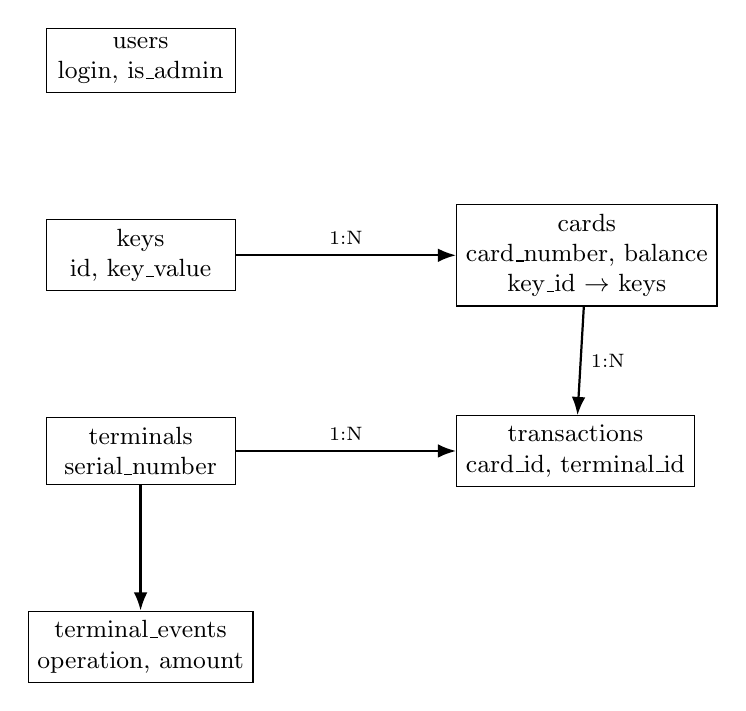
\begin{tikzpicture}[
    ent/.style={draw, align=center, minimum width=2.4cm, font=\small},
    rel/.style={-{Latex}, thick}
  ]
    \node[ent] (keys) {keys\\id, key\_value};
    \node[ent, right=2.8cm of keys] (cards) {cards\\card\_number, balance\\key\_id $\rightarrow$ keys};
    \node[ent, below=1.6cm of keys] (term) {terminals\\serial\_number};
    \node[ent, right=2.8cm of term] (txn) {transactions\\card\_id, terminal\_id};
    \node[ent, below=1.6cm of term] (tev) {terminal\_events\\operation, amount};
    \node[ent, above=1.6cm of keys] (usr) {users\\login, is\_admin};

    \draw[rel] (keys) -- node[above, font=\scriptsize]{1:N} (cards);
    \draw[rel] (cards) -- node[right, font=\scriptsize]{1:N} (txn);
    \draw[rel] (term) -- node[above, font=\scriptsize]{1:N} (txn);
    \draw[rel] (term.south) -- ++(0,-0.3) -| (tev.north);
  \end{tikzpicture}
  \caption{Логическая схема связей таблиц SQLite}
  \label{fig:er}
\end{figure}

\texttt{cards} хранит номер карты, баланс, флаг блокировки и ссылку на ключ.
\texttt{transactions} фиксирует сумму, карту и терминал.
При событиях \texttt{debit\_card} и \texttt{credit\_balance} баланс обновляется внутри одной транзакции БД.
\texttt{terminal\_events} используется для журнала терминала; SPA получает новые записи через \texttt{GET /terminal/events?since=} каждые 2~с.

\section{API бэкенда}

REST API версии~v1 документирован в Swagger~\cite{swaggo}.
Базовый префикс: \texttt{https://localhost:8888/api/v1}.
Основные группы эндпоинтов приведены в таблице~\ref{tab:api}.

\begin{table}[H]
  \centering
  \caption{Основные группы API}
  \label{tab:api}
  \small
  \begin{tabular}{|l|p{9.5cm}|}
    \hline
    \textbf{Группа} & \textbf{Назначение} \\
    \hline
    \texttt{auth} & \texttt{POST /auth/login}~--- JWT пользователя; \texttt{GET /me}~--- профиль \\
    \hline
    \texttt{terminal} & \texttt{POST /terminal/auth/login}; \texttt{POST /terminal/authorize} (решение без списания); \texttt{GET /terminal/keys}; \texttt{POST /terminal/register-card}; \texttt{POST /terminal/event}; \texttt{GET /terminal/events} \\
    \hline
    \texttt{cards}, \texttt{terminals}, \texttt{transactions} & CRUD для авторизованных пользователей \\
    \hline
    \texttt{keys}, \texttt{users} & CRUD только для администратора \\
    \hline
  \end{tabular}
\end{table}

\texttt{/terminal/authorize} проверяет терминал, карту, блокировку и достаточность баланса, возвращая \texttt{\{approved, reason\}}.
Фактическое изменение баланса выполняется при событии \texttt{debit\_card}; так сервер остаётся арбитром, а карта хранит локальную копию баланса.

\begin{figure}[H]
  \centering
  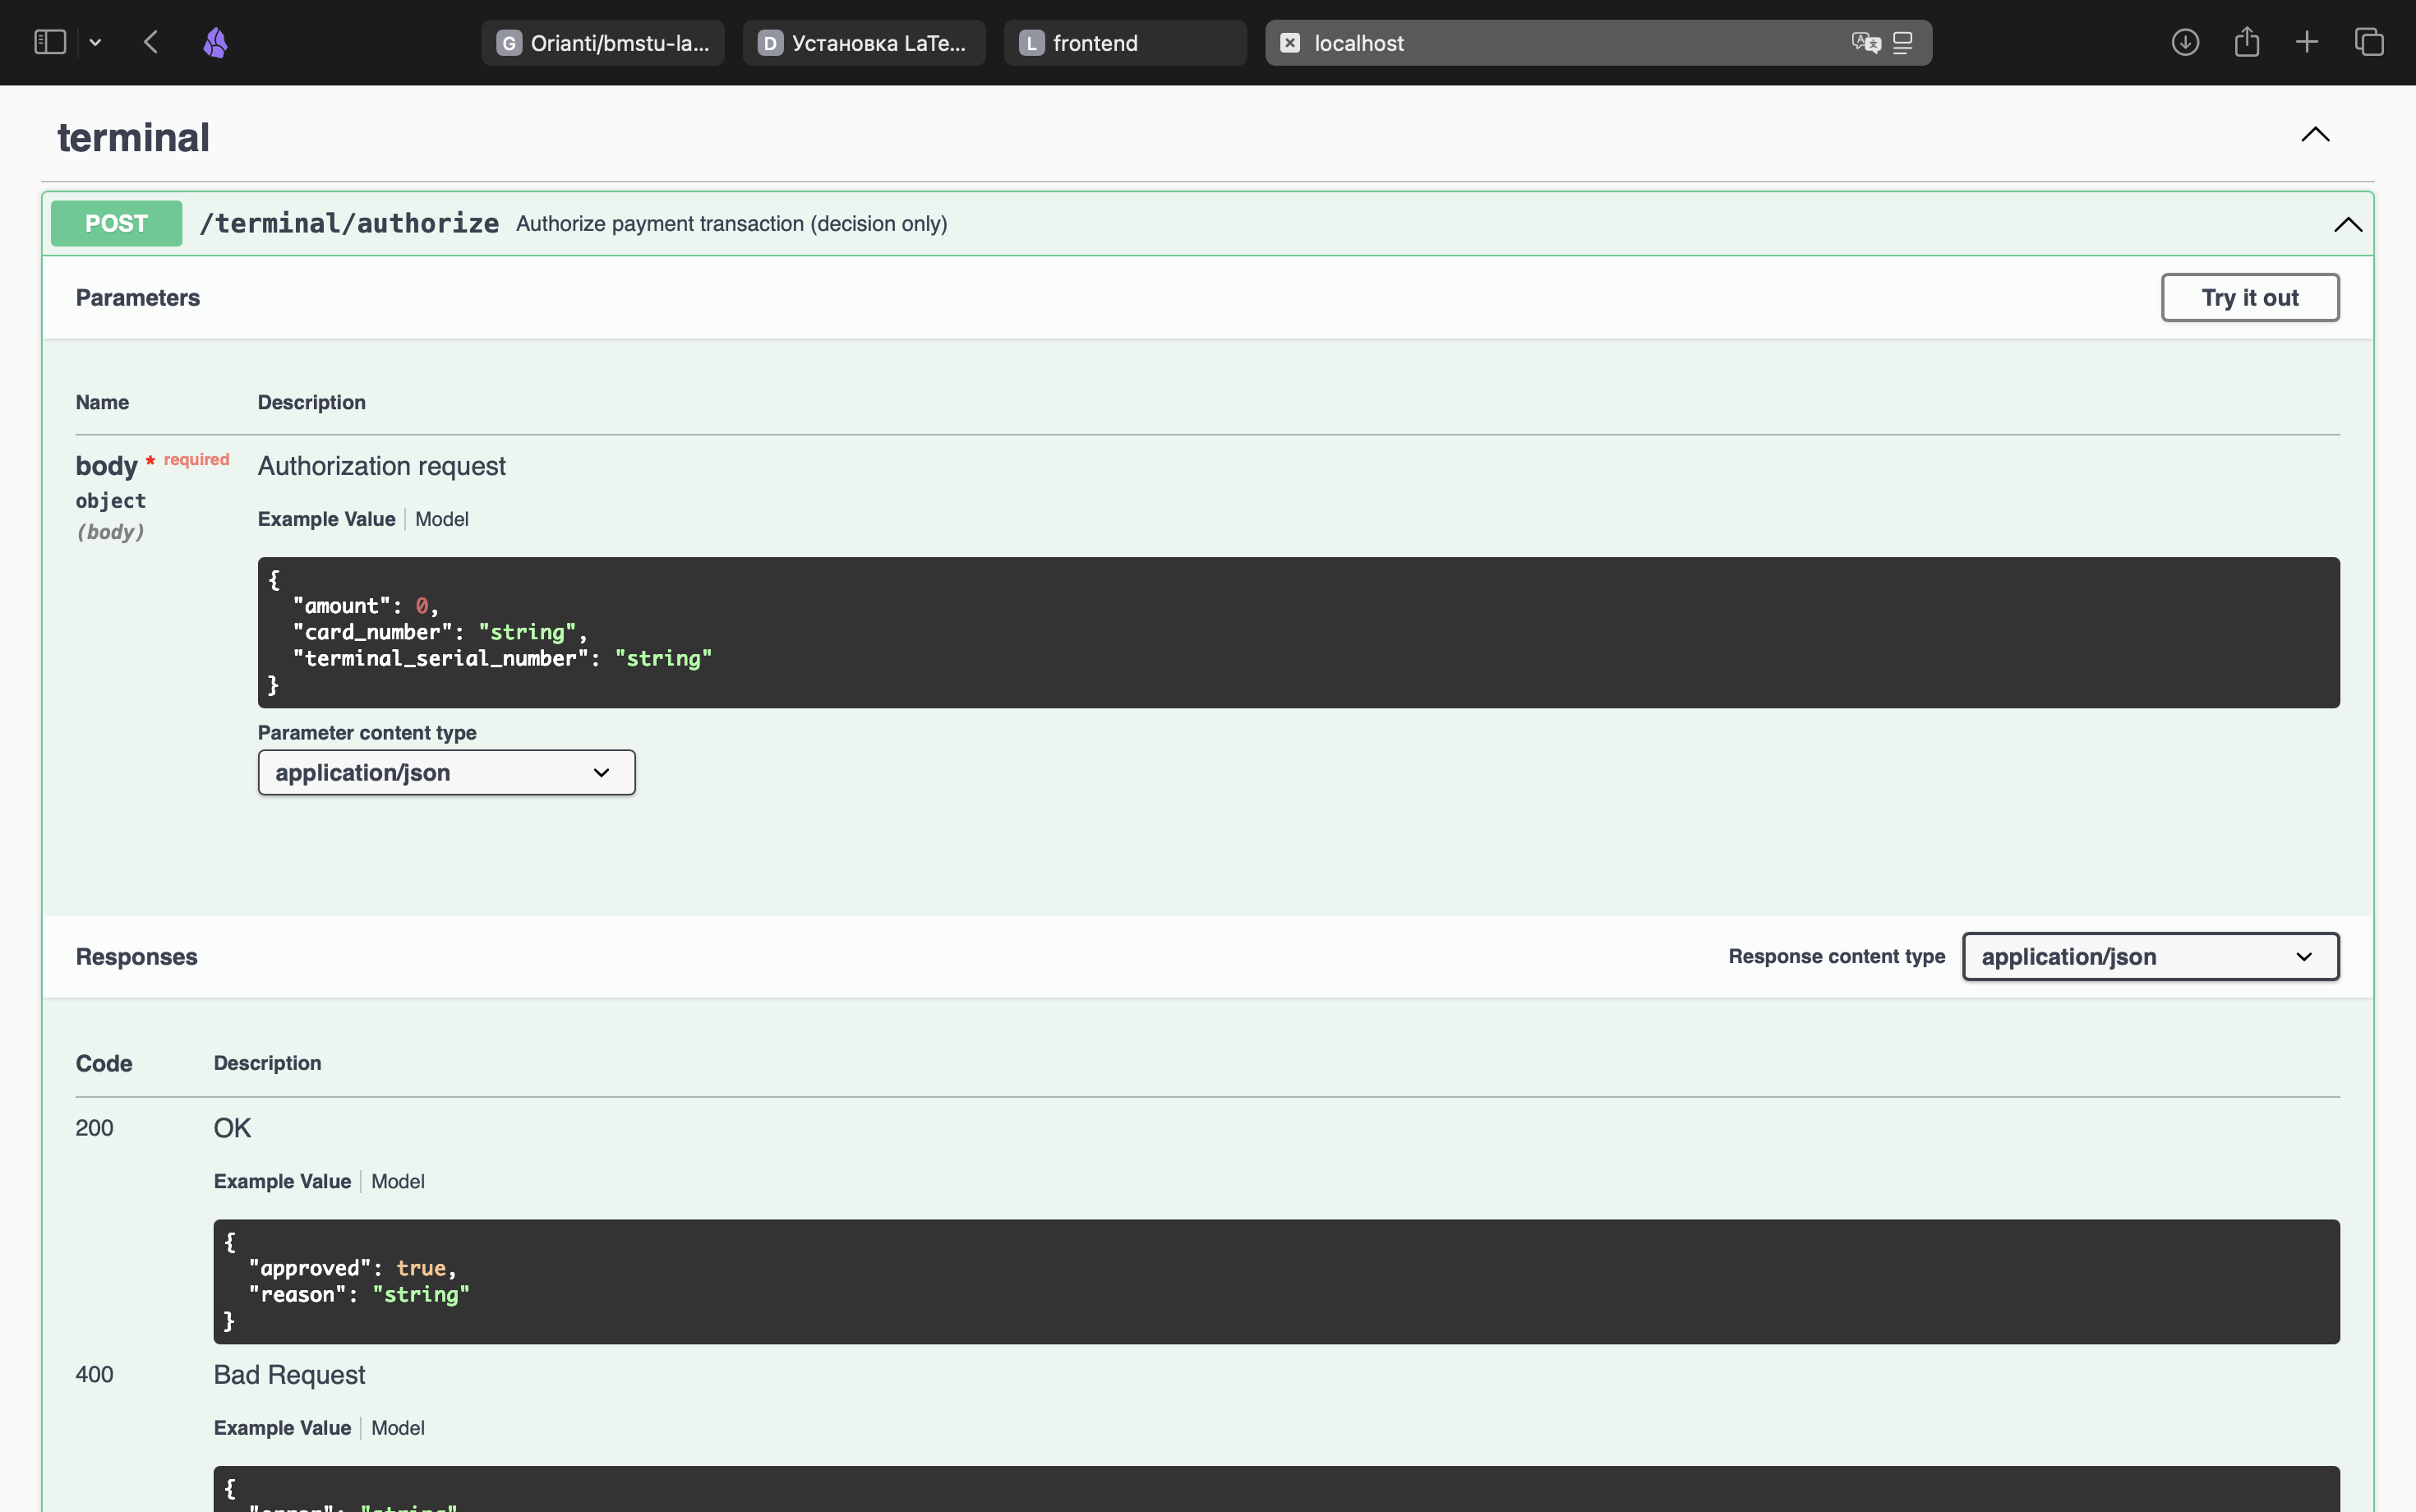
\includegraphics[width=0.88\textwidth]{images/swagger-terminal-authorize.png}
  \caption{Описание эндпоинта авторизации в Swagger UI}
  \label{fig:swagger-authorize}
\end{figure}

\section{Фронтенд}

Клиентская часть написана на React и TypeScript, сборка выполняется Vite, интерфейс собран на Material UI~\cite{mui,react}.
Есть страница входа \texttt{/login} и защищённая зона с боковым меню: карты, терминалы, транзакции, ключи и пользователи.
\texttt{CrudTable} и \texttt{EntityDialog} используются на большинстве страниц, поэтому таблицы и формы не дублируются вручную.
Структура экранов показана на рис.~\ref{fig:ui-structure}; на странице «Терминалы» отдельно показан live-журнал NFC-операций (рис.~\ref{fig:ui-mock}).
Для администратора владелец карты выбирается из списка пользователей, обычный пользователь вводит имя вручную.

\begin{figure}[H]
  \centering
  \begin{tikzpicture}[
    node distance=0.85cm and 1.0cm,
    screen/.style={draw, rounded corners, minimum width=2.2cm, minimum height=0.7cm, font=\scriptsize, align=center},
    admin/.style={screen, fill=gray!10},
    arr/.style={-{Latex}}
  ]
    \node[screen] (login) {Вход\\\texttt{/login}};
    \node[admin, right=of login] (layout) {Защищённая зона\\\texttt{AppLayout}};
    \node[screen, above right=0.45cm and 0.9cm of layout] (terminals) {Терминалы\\+ журнал};
    \node[screen, right=of terminals] (cards) {Карты};
    \node[screen, below=of cards] (transactions) {Транзакции};
    \node[screen, below right=0.45cm and 0.9cm of layout] (keys) {Ключи};
    \node[screen, right=of keys] (users) {Пользователи};

    \draw[arr] (login) -- node[above, font=\scriptsize]{JWT} (layout);
    \draw[arr] (layout) -- (terminals);
    \draw[arr] (layout) -- (cards);
    \draw[arr] (layout) -- (transactions);
    \draw[arr] (layout) -- (keys);
    \draw[arr] (layout) -- (users);
  \end{tikzpicture}
  \caption{Структура экранов веб-интерфейса}
  \label{fig:ui-structure}
\end{figure}

\begin{figure}[H]
  \centering
  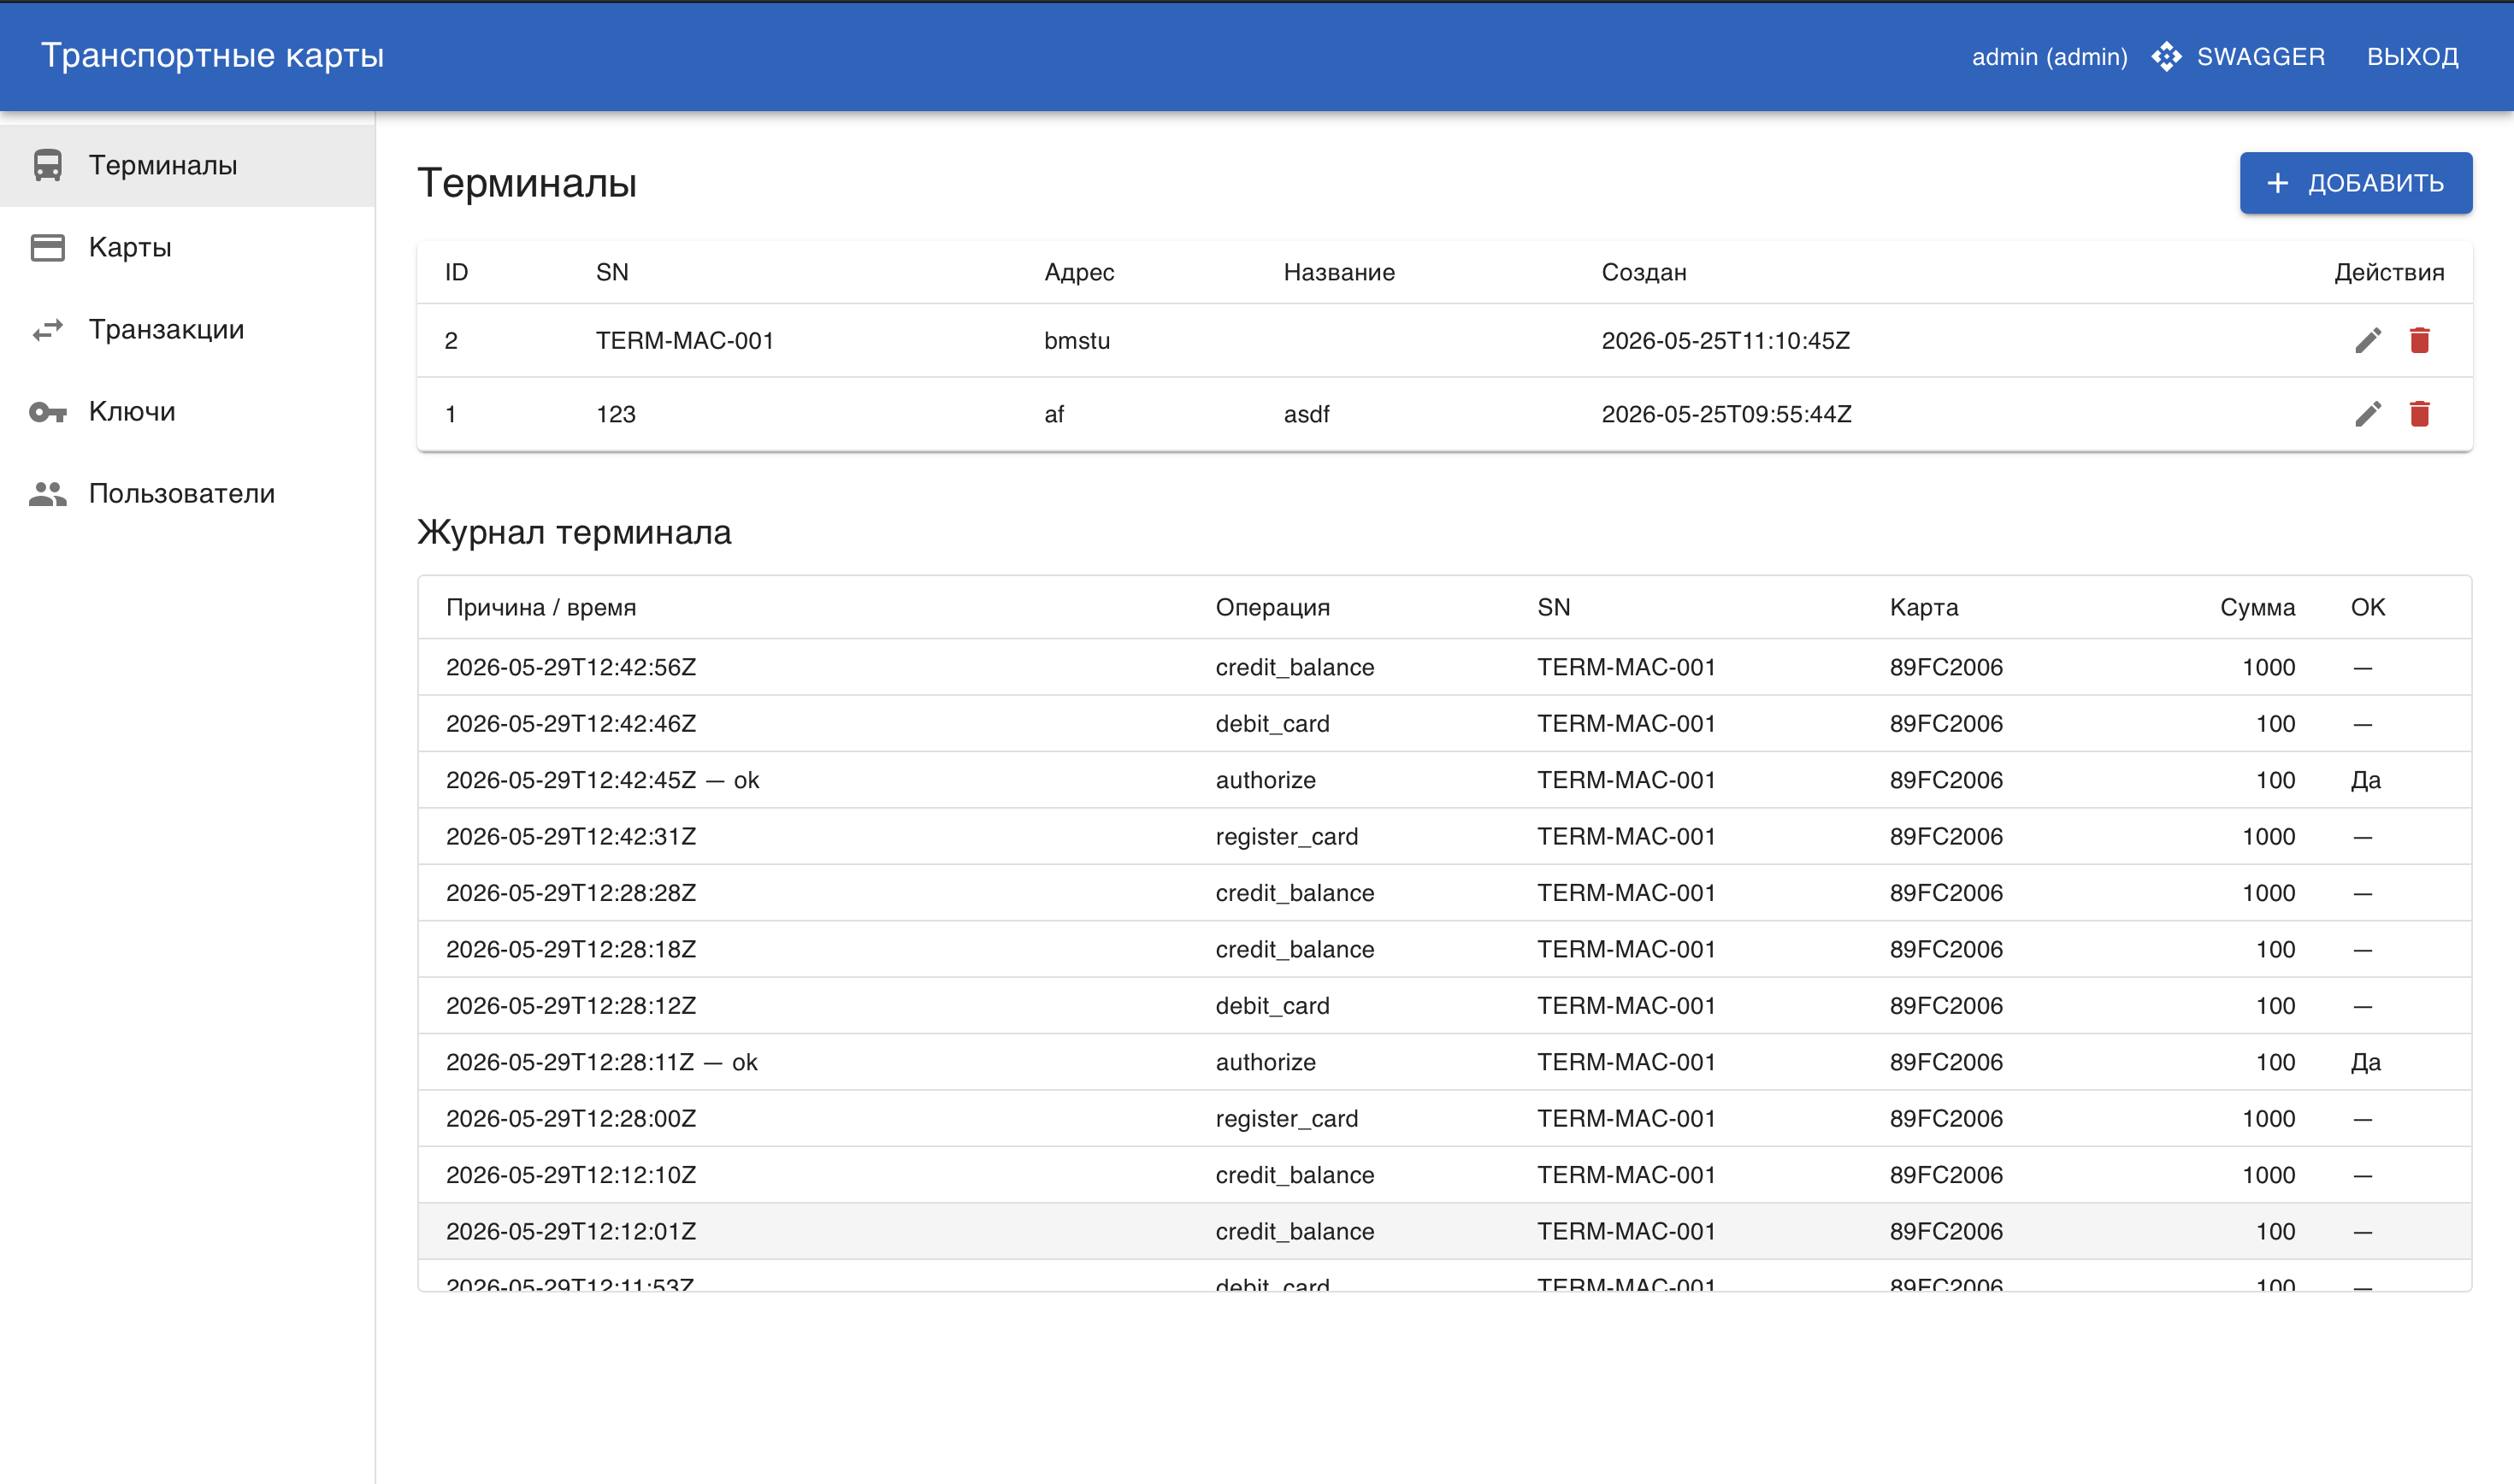
\includegraphics[width=0.88\textwidth]{images/spa-terminals.png}
  \caption{Фрагмент веб-интерфейса}
  \label{fig:ui-mock}
\end{figure}

\section{Клиент. Взаимодействие с аппаратурой}

Терминальное приложение написано на Flutter и запускается на macOS.
Работа с ридером вынесена в C-модуль \texttt{nfc\_card.c}; он линкуется в Runner и вызывается из Dart через FFI~\cite{flutter_ffi}.

\textbf{Подключение библиотек:}
\begin{enumerate}
  \item установлены зависимости Homebrew: \texttt{libnfc}, \texttt{openssl@3};
  \item в \texttt{NfcNative.xcconfig} указаны include/lib пути и флаги \texttt{-lnfc -lssl -lcrypto};
  \item \texttt{nfc\_card.c} и \texttt{mifare\_compat.c} добавлены в macOS Runner;
  \item \texttt{NfcBridge} загружает функции \texttt{nfc\_read\_card}, \texttt{nfc\_write\_card}, \texttt{nfc\_reader\_present};
  \item ожидание карты выполняется в \texttt{Isolate.run}, чтобы интерфейс не зависал.
\end{enumerate}

В терминале есть вкладки «Регистрация», «Карта», «Списание», «Пополнение».
При старте приложение логинится через \texttt{POST /terminal/auth/login}, загружает ключи с \texttt{GET /terminal/keys} и проверяет ридер функцией \texttt{nfc\_reader\_present()}.

\begin{figure}[H]
  \centering
  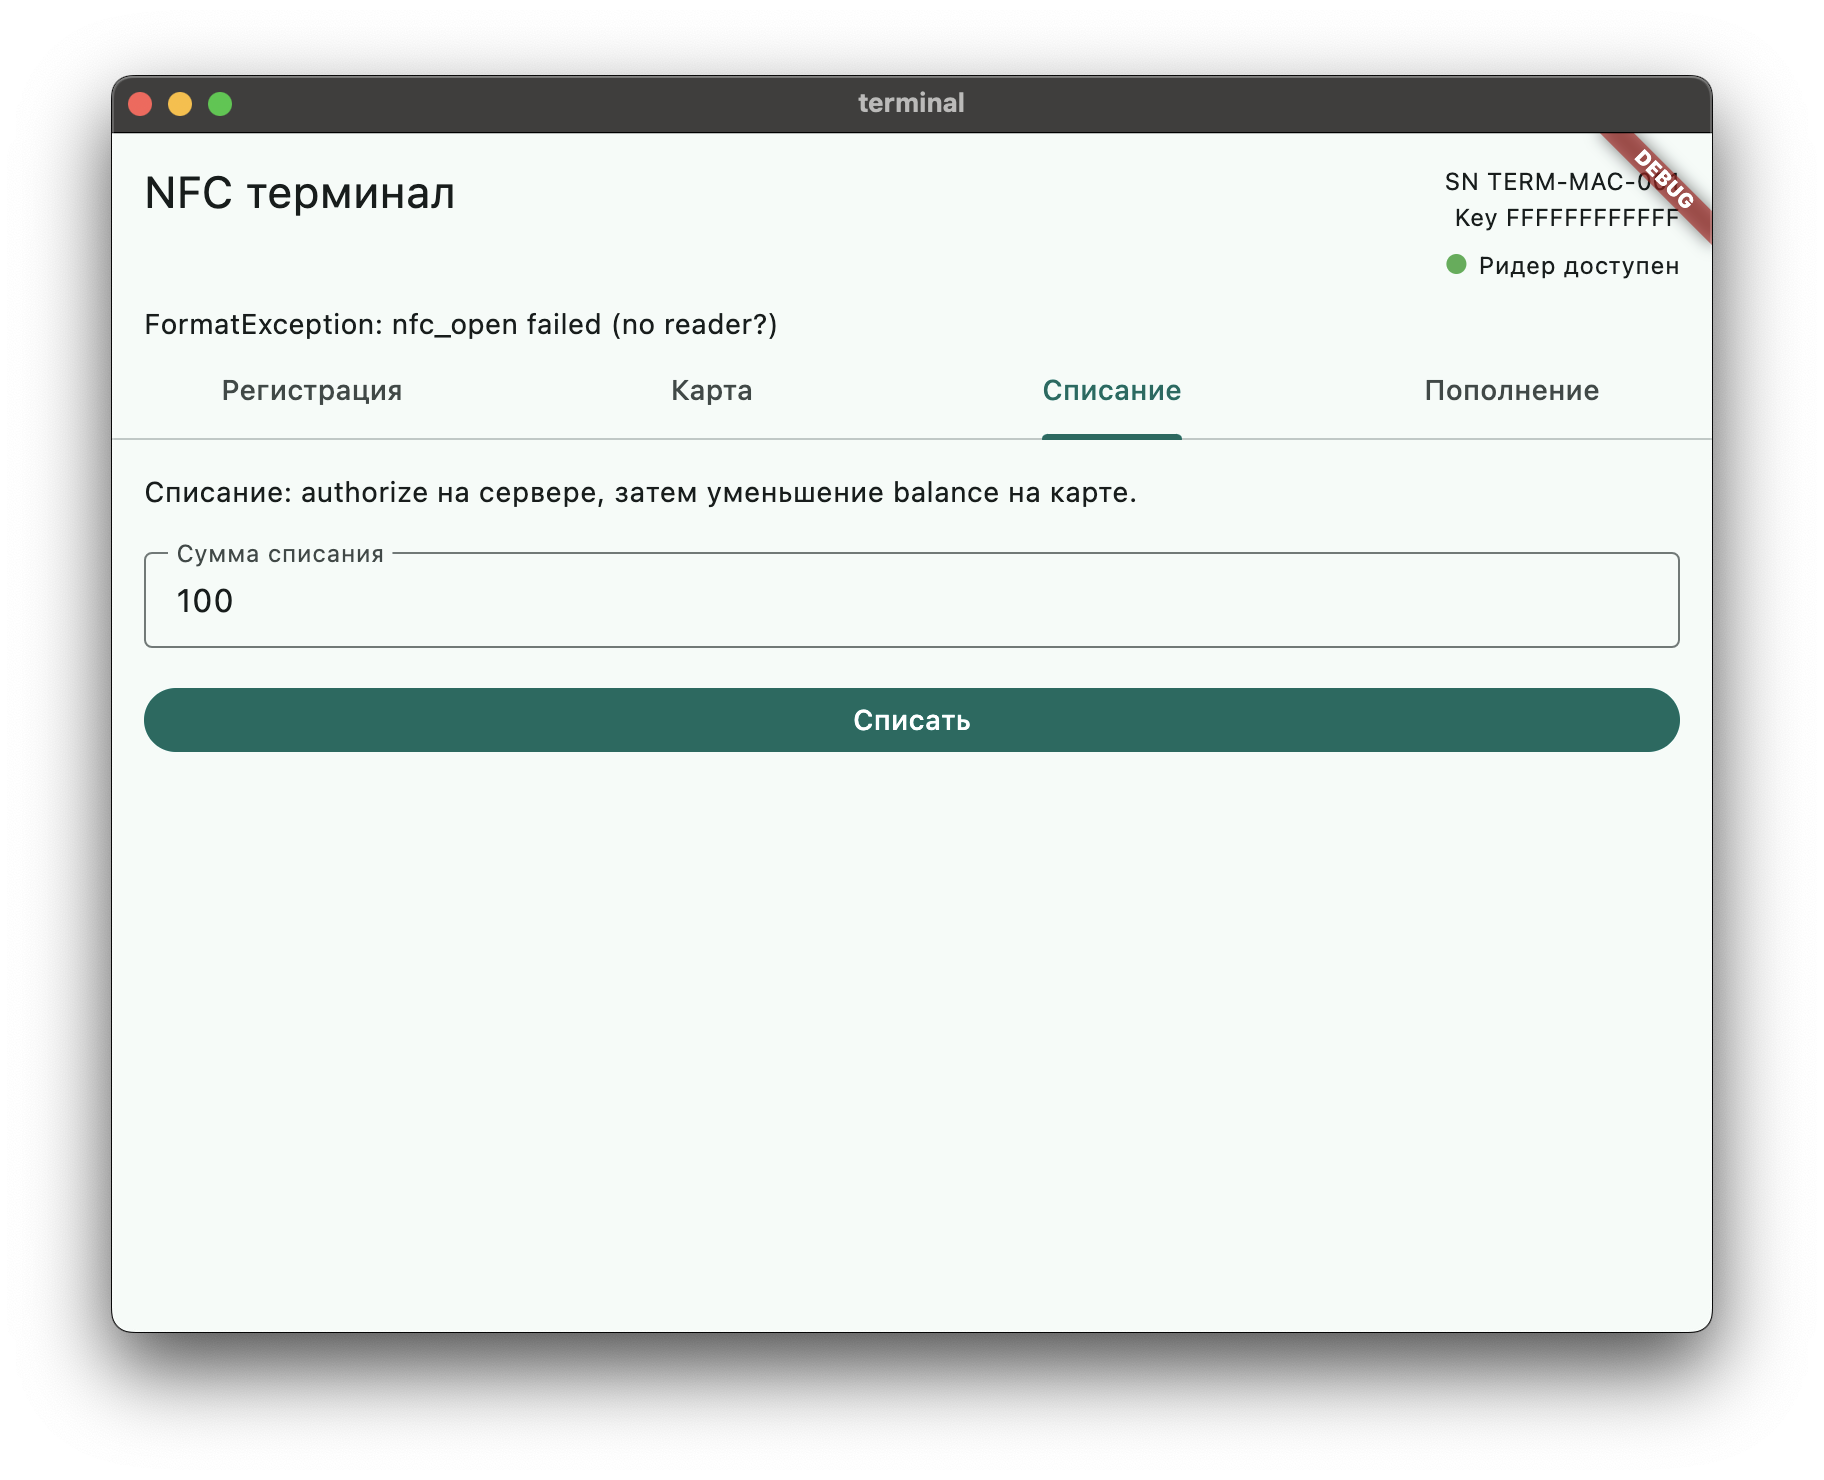
\includegraphics[width=0.88\textwidth]{images/flutter-debit.png}
  \caption{Интерфейс NFC-терминала}
  \label{fig:term-mock}
\end{figure}

\section{Фрагменты кода}

Проверка платежа на сервере:

\begin{lstlisting}[frame=single]
if _, err := (store.Terminals{DB: s.DB}).GetBySerialNumber(
    r.Context(), req.TerminalSerialNumber); err != nil {
    writeError(w, http.StatusInternalServerError, "internal", "database error")
    return
}

card, err := (store.Cards{DB: s.DB}).GetByCardNumber(r.Context(), req.CardNumber)
if err != nil {
    writeError(w, http.StatusInternalServerError, "internal", "database error")
    return
}

if card.IsBlocked {
    resp = terminalAuthorizeResponse{Approved: false, Reason: "card_blocked"}
} else if card.Balance < req.Amount {
    resp = terminalAuthorizeResponse{Approved: false, Reason: "insufficient_funds"}
} else {
    resp = terminalAuthorizeResponse{Approved: true, Reason: "ok"}
}
\end{lstlisting}

Запись блоков MIFARE с аутентификацией и шифрованием:

\begin{lstlisting}[frame=single]
uint8_t aes_key[16];
derive_aes_key(mifare_key, aes_key);

for (int i = 0; i < DATA_BLOCK_COUNT; i++) {
  uint8_t block = k_data_blocks[i];
  if (mifare_auth(session->dev, nt, block, mifare_key) != NFC_CARD_OK) {
    return NFC_CARD_ERR;
  }
  mifare_param mp;
  uint8_t wire[BLOCK_SIZE];
  const uint8_t *src = plain + i * BLOCK_SIZE;
  if (encrypt_block_aes(aes_key, src, wire) != NFC_CARD_OK) {
    return NFC_CARD_ERR;
  }
  memcpy(mp.mpd.abtData, wire, BLOCK_SIZE);
  if (!nfc_initiator_mifare_cmd(session->dev, MC_WRITE, block, &mp)) {
    set_error("mifare write failed");
    return NFC_CARD_ERR;
  }
}
\end{lstlisting}

Вызов C-функции из Dart через FFI:

\begin{lstlisting}[frame=single]
final keyPtr = _allocUtf8(mifareKeyHex);
final uidBuf = calloc<ffi.Uint8>(64);
final jsonBuf = calloc<ffi.Uint8>(1024);
try {
  final rc = _nfcReadCard(keyPtr, uidBuf, 64, jsonBuf, 1024);
  if (rc != 0) {
    throw FormatException(lastLibError());
  }
  return (
    uid: _peekUtf8Zeros(uidBuf, 64),
    json: _peekUtf8Zeros(jsonBuf, 1024),
  );
} finally {
  calloc.free(keyPtr);
  calloc.free(uidBuf);
  calloc.free(jsonBuf);
}
\end{lstlisting}

Регистрация терминальных маршрутов API:

\begin{lstlisting}[frame=single]
mux.Handle("POST /api/v1/terminal/authorize",
          terminalAuthed(s.handleTerminalAuthorize))
mux.Handle("GET /api/v1/terminal/keys",
          terminalAuthed(s.handleTerminalKeys))
mux.Handle("POST /api/v1/terminal/event",
          terminalAuthed(s.handleTerminalEventPost))
mux.Handle("POST /api/v1/terminal/register-card",
          terminalAuthed(s.handleTerminalRegisterCard))
\end{lstlisting}

\chapter{Тестирование}

Функциональное тестирование я выполнял вручную: сервер запускался через Docker Compose, терминал~--- через Flutter на macOS.

\begin{enumerate}
  \item \textbf{Развёртывание:} \texttt{docker compose up --build}, затем проверка \texttt{/health} и Swagger.
  \item \textbf{Админка:} вход \texttt{admin/admin}, создание ключа MIFARE и терминала \texttt{TERM-MAC-001}.
  \item \textbf{Терминал:} \texttt{flutter run -d macos}, регистрация карты и чтение баланса.
  \item \textbf{Списание:} успешный debit при согласованном балансе карты и БД.
  \item \textbf{Отказ:} сумма выше баланса возвращает \texttt{approved=false} и \texttt{insufficient\_funds}.
  \item \textbf{Пополнение:} \texttt{credit\_balance} увеличивает баланс на карте и в БД.
\end{enumerate}

\begin{figure}[H]
  \centering
  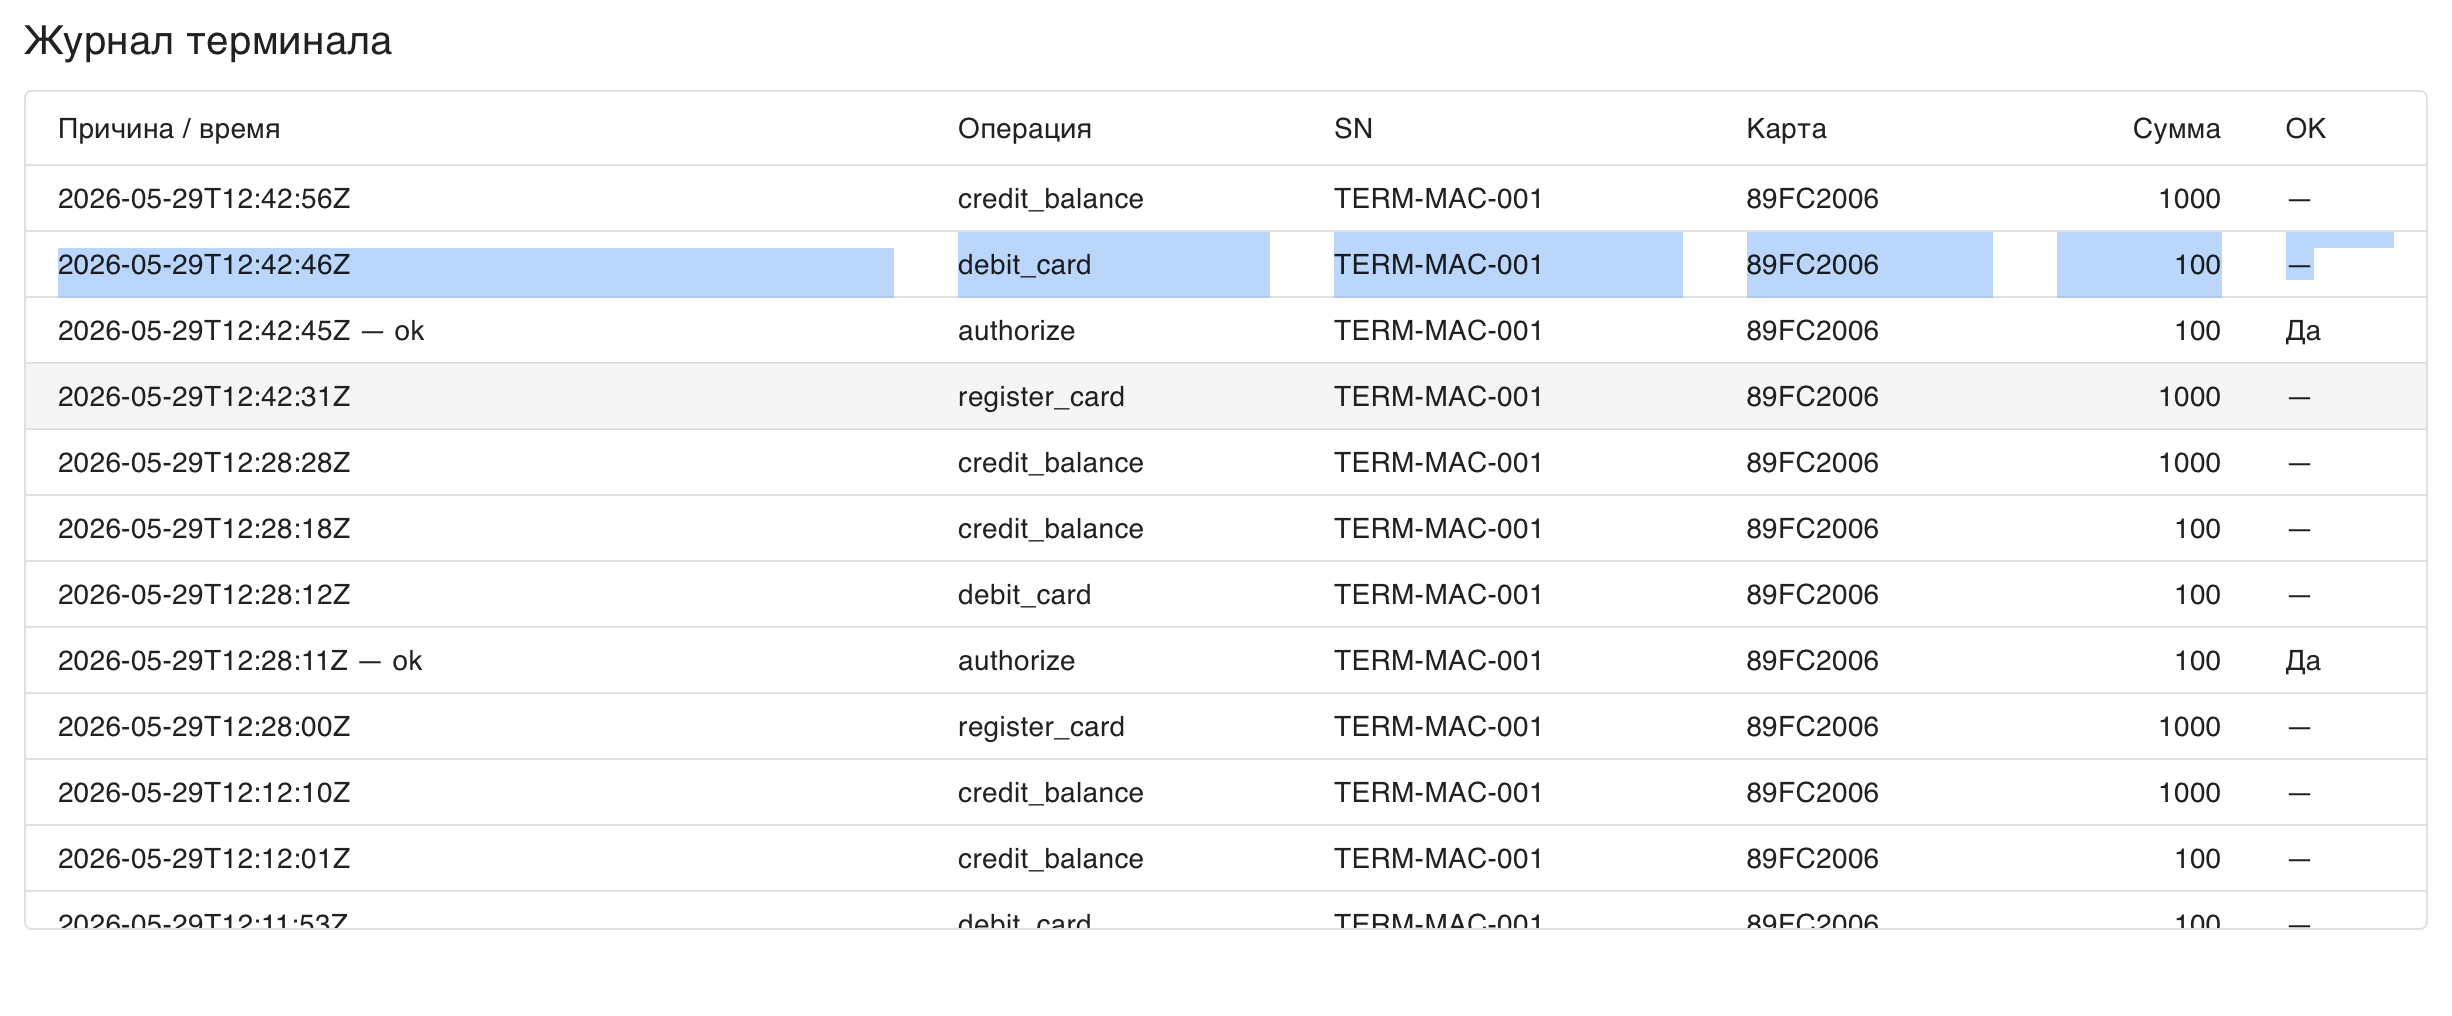
\includegraphics[width=0.88\textwidth]{images/terminal-journal-debit.png}
  \caption{Результат ручного теста}
  \label{fig:test-mock}
\end{figure}

Основные сценарии прошли успешно.
Ошибки чтения карты выводятся в статусной строке терминала через \texttt{nfc\_last\_error()}.

\chapter{Заключение}

В результате лабораторных работ получился работающий прототип:
\begin{itemize}
  \item сервер авторизации на Go с SQLite, JWT и Swagger-документацией;
  \item веб-админка на React/MUI с CRUD и журналом терминала;
  \item macOS-терминал на Flutter с FFI-доступом к PN532 через libnfc;
  \item формат хранения данных на MIFARE Classic с AES-шифрованием блоков.
\end{itemize}

Система запускается через Docker Compose и показывает полный цикл: запись карты, авторизация платежа, изменение баланса на носителе и появление событий в веб-интерфейсе.

\makebibliography

\end{document}
